
\subsubsection{Modell}
Die nummerische Analyse findet mit Hilfe des Programms ABAQUS des Anbieters Dassault Systemes statt. Das Programm ist für Studenten kostenlos erhältlich, jedoch ist diese Version auf eine Anzahl von 1000 Knoten beim Vernetzen des Bauteils beschränkt.\\
Das zuvor erstellte CAD-Modell wird zunächst in ABAQUS importiert. Da es sich nun noch um ein Bauteil aus Vollmaterialien handelt und für eine möglichst genaue Analyse ein Schalenmodell verwendet werden soll, muss das Modell zunächst umgewandelt werden. Dafür werden die Volumenkörper des Modells in zweidimensionale Flächen umgewandelt, denen im Folgenden dann eine Dicke zugeortnet werden kann (siehe Abb.\ref{Schalenmodell}).

\begin{figure}[h]
 \centering
 \includegraphics[scale=0.4]{Bilder/Flügel_ABAQUS}
 \caption{Schalenmodell}
 \label{Schalenmodell}
\end{figure}
\newpage
\noindent
Daraufhin werden die Kennwerte der Materialien in das Programm integriert. Hierbei werden die Werte für GFK, den Schaum und die Rippen eingetragen (siehe Abb.\ref{Material}).Diese wurden in Kapitel 4.3.1 mit Hilfe von elamX festgelegt. Für GFK wird das Material als Laminat erstellt, wodurch der E-Modul parallel und senkrecht zur Faser, sowie die Schubmodule definiert werden können.\\
\noindent
Nun wird das Schalenmodell in die Verschiedenen Segmente Unterteilt , denen dann Materialien und deren entsprechenden Dicken und Anzahl von Schichten zugeortnet werden. Hierbei wird das Bauteil in den dicken und den dünnen Teil des Stegs, die Gurte, die Haut, sowie die Rippen unterteilt. Für die Bauteile aus GFK werden erst zwei zum Flügelkoordinatensystem um 45 und -45 Grad gedrehte GFK-Schichten definiert(siehe Abb. \ref{Steg_Material}), dann der Schaum und daraufhin erneut zwei versetzte GFK-Schichten. Eine Schicht hat hierbei ein Viertel der zuvor berechneten Dicke ohne des Schaums. Für die Rippen wird eine Dicke von 3mm angenommen.\\
\noindent
Als nächstes werden die Randbedingungen und Angreifenden Kräfte festgelegt. Der Holm ist in der Einspannung fest gelagert. Daher wird an der Stelle der Lager A und B eine feste Einspannung angenommen. Die Aufgenommenen Kräfte durch die Querkraftbolzen werden als Kräfte angebracht.Die Prüfkraft wird am L/4-Punkt eingeleitet.\\
Daraufhin wird das Bauteil vernetzt. Hierbei wird eine Anzahl an Knoten pro Längeneinheit eingegeben und das Programm verbindet diese zu einem Netz aus Flächen.Durch die Begrenzung auf 1000 Knoten ist das Netz jedoch recht grob. \\
\newpage
\subsubsection{Analyse}
Zunächst wird eine Prüfkraft von 100N angelegt, um die maximale Absenkung zu ermitteln. Hierbei ergibt sich für die Absenkung $z_{max}=17,34mm$, welche erwartungsgemäß an der Spitze des Flügels auftritt. Dies ist weniger als die geforderte Absenkung von $z_{max}=22mm$ und somit kann dieses Aufgabenkriterium als erfüllt angesehen werden.(siehe Abb.\ref{Absenkung})
\begin{figure}[h]
 \centering
 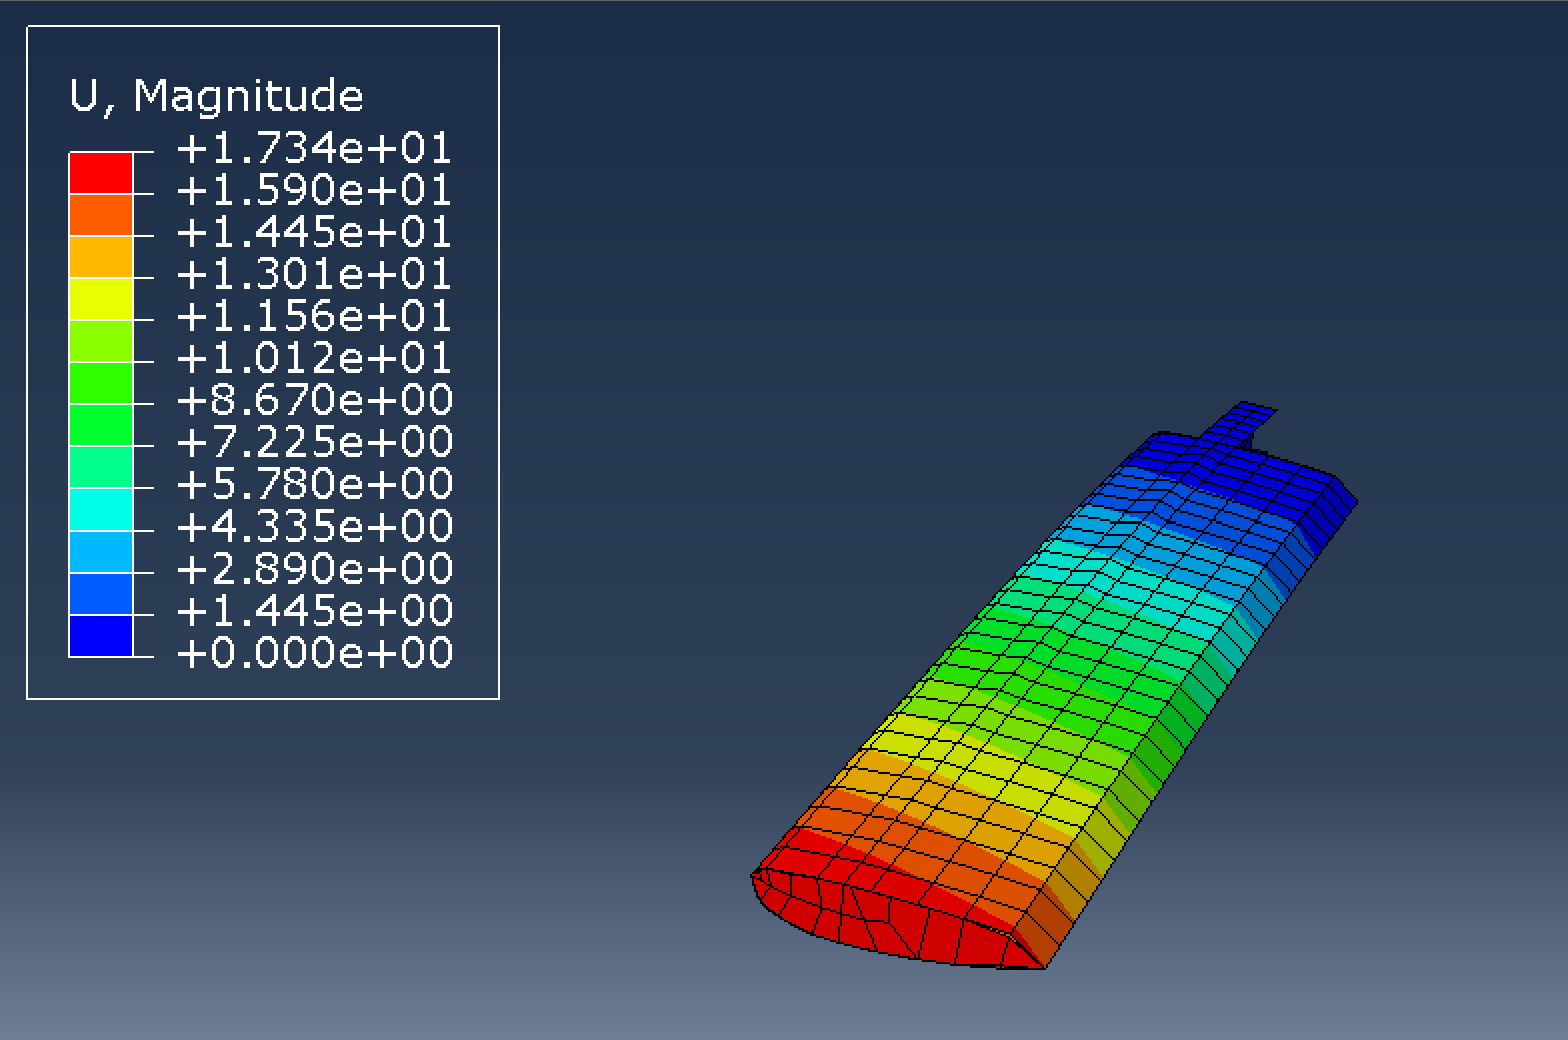
\includegraphics[scale=0.4]{Bilder/Absenkung_100N}
 \caption{Absenkung bei einer Belastung von 100N}
 \label{Absenkung}
\end{figure}
\newpage
\noindent
Um herauszufinden, ob der Flügel eine hinreichende Festigkeit aufweist wird die Prüfkraft auf 500N erhöht. Nun müssen die maximalen Spannungen im Bauteil mit den Kennwerten verglichen werden. Das Modell zeigt nun maximale Spannungen an der Stelle des Lagers B an. Da sich dort allerdings noch eine nicht mit modellierte Verstärkung durch Holzblöcke befindet sind diese Werte deutlich höher als in der Realität. Daher werden nur die Werte betrachtet, die sich ab der Rippe ergeben.\\
Die maximale Vergleichsspannung ergibt sich im Steg des Holms. Die Normalspannung in $x_{1}$-Richtung ist im vorderen Teil des Stegs am höchsten und beträgt beim Maximum $85,63\frac{N}{mm^2}$.\\
Die Normalspannung in $x_{2}$-Richtung ist im Gurt der Unterseite des Flügels (im Veruchsaufbau Oberseite) und beträgt maximal $14,25\frac{N}{mm^2}$.Die Spannung in $x_{3}$-Richtung ist überall 0.\\
Die Schubspannung ist in der Schale auf der Unterseite am höchsten. Hier ergibt sich ein Maximalwert von $16,72\frac{N}{mm^2}$.\\
\noindent
Das Angenommene Koordinatensystem bezieht ich auf die oberste Schicht des Laminats. Daher sind $x_{1}$ und $x_{2}$ immer in Richtung der Faser oder orthogonal dazu.\\
Da die Spannungen nicht in allen Schichten gleich seinen müssen haben die Spannungen allerdings eine geringe Aussagekraft. Eine bessere Aussage lässt sich durch die maximale Dehnungen in den einzelnen Koordinatenrichtungen treffen. Durch die Annahme, dass die Dehnung in allen schichten gleich ist, kann diese in elamX eingegeben werden und so eine Sicherheit gegen Bruch ermittelt werden.

\begin{center}
\begin{tabular}[h]{l|c|c}
Koordinatenrichtung&Dehnung&Sicherheit\\
\hline
$x_{1}$&10,253&1\\
$x_{2}$&2,0506&1\\
$x_{3}$&1,0253&1\\
\end{tabular}
\end{center}

Die Werte sind durch das Zusammenspiel aller Bauteile sehr viel kleiner als in den Vorherigen Berechnungen. Dadurch bestätigt das FEM- Modell die vorangegangenen Berechnungen.
\newpage
\subsubsection{Beulanalyse}
Da der Holmstummel bis zum Lager C nicht ausreichend modelliert werden konnte wird für die Beulauslegung eine feste Einspannung am Lager C angenommen (siehe Abb.\ref{BEinspannung}).
\begin{figure}[h]
 \centering
 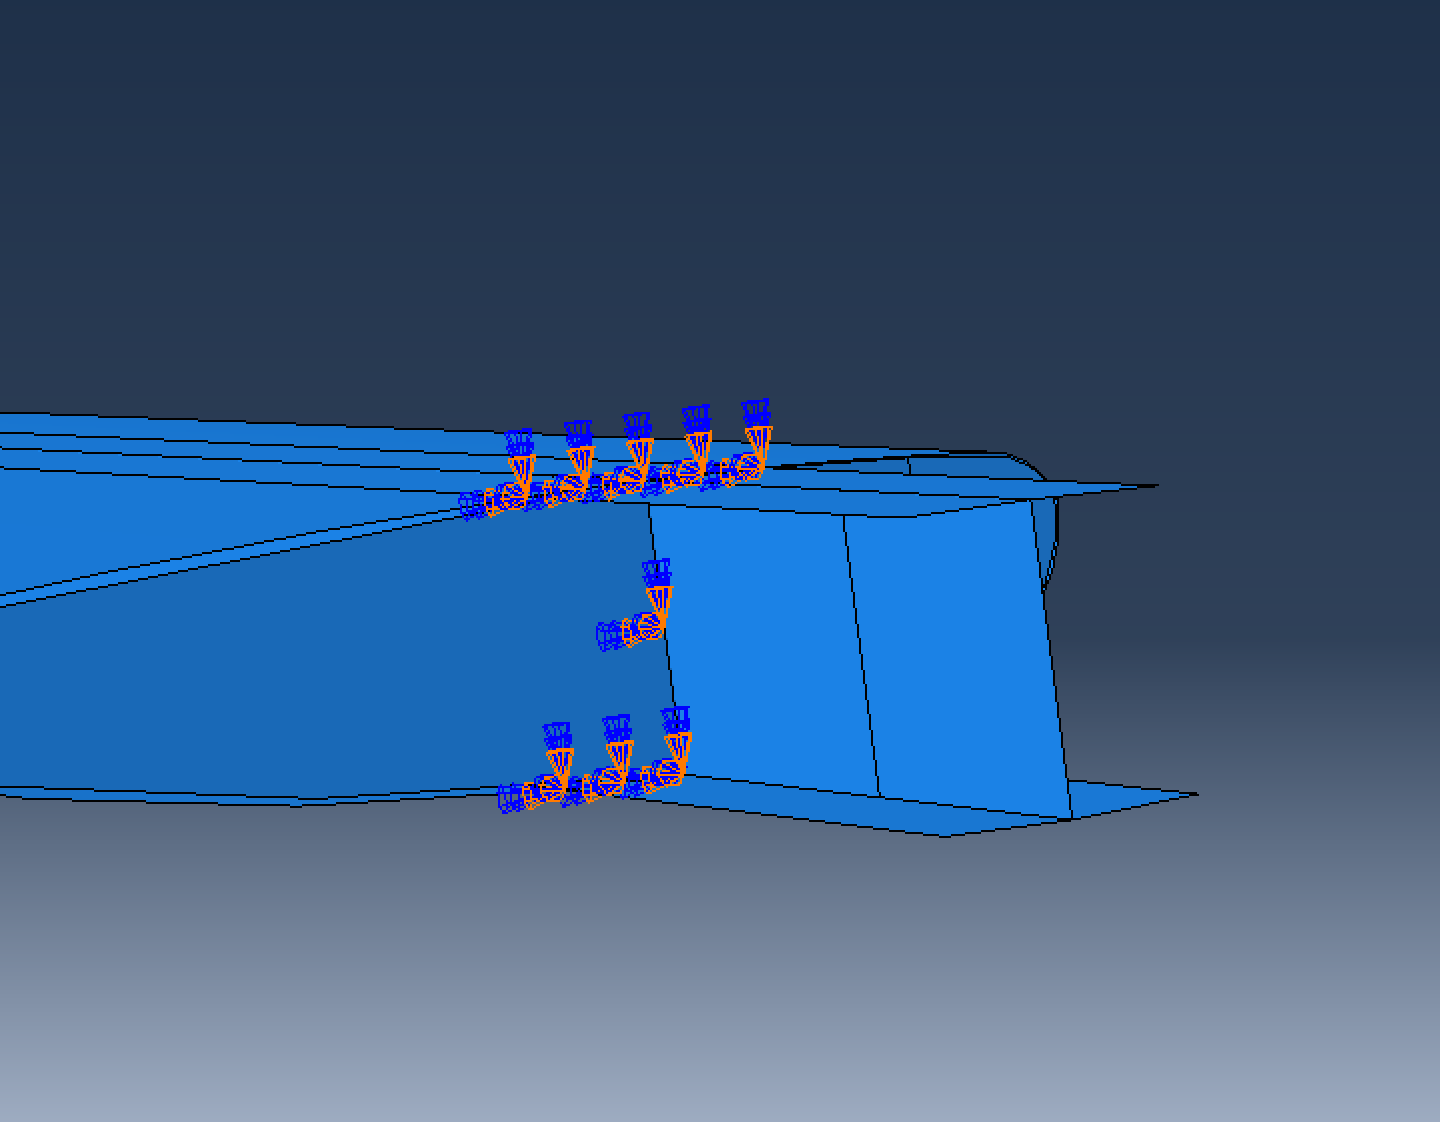
\includegraphics[scale=0.4]{Bilder/Beuleinspannung}
 \caption{Einspannung am Lager C}
 \label{BEinspannung}
\end{figure}
\noindent
Nun können die Eigenwerte für die Belastung von 100N, 500N und 1000N abgelesen werden.
\begin{center}
\begin{tabular}[h]{l|c}
Prüfkraft&Beulfaktor\\
\hline
100N&10,253\\
500N&2,0506\\
1000N&1,0253\\
\end{tabular}
\end{center}
\noindent
Diese Werte sind alle größer als 1, damit ist der Flügel für alle drei Belastungsfällen ausreichend gegen das Beulen dimensioniert.
Das Programm ermöglicht außerdem die Ausgabe möglicher Beulformen. Ein Beispiel in Abbildung \ref{Beulform} dargestellt. Die Haut würde nah am Holmstummel beulen. 
\begin{figure}[h]
 \centering
 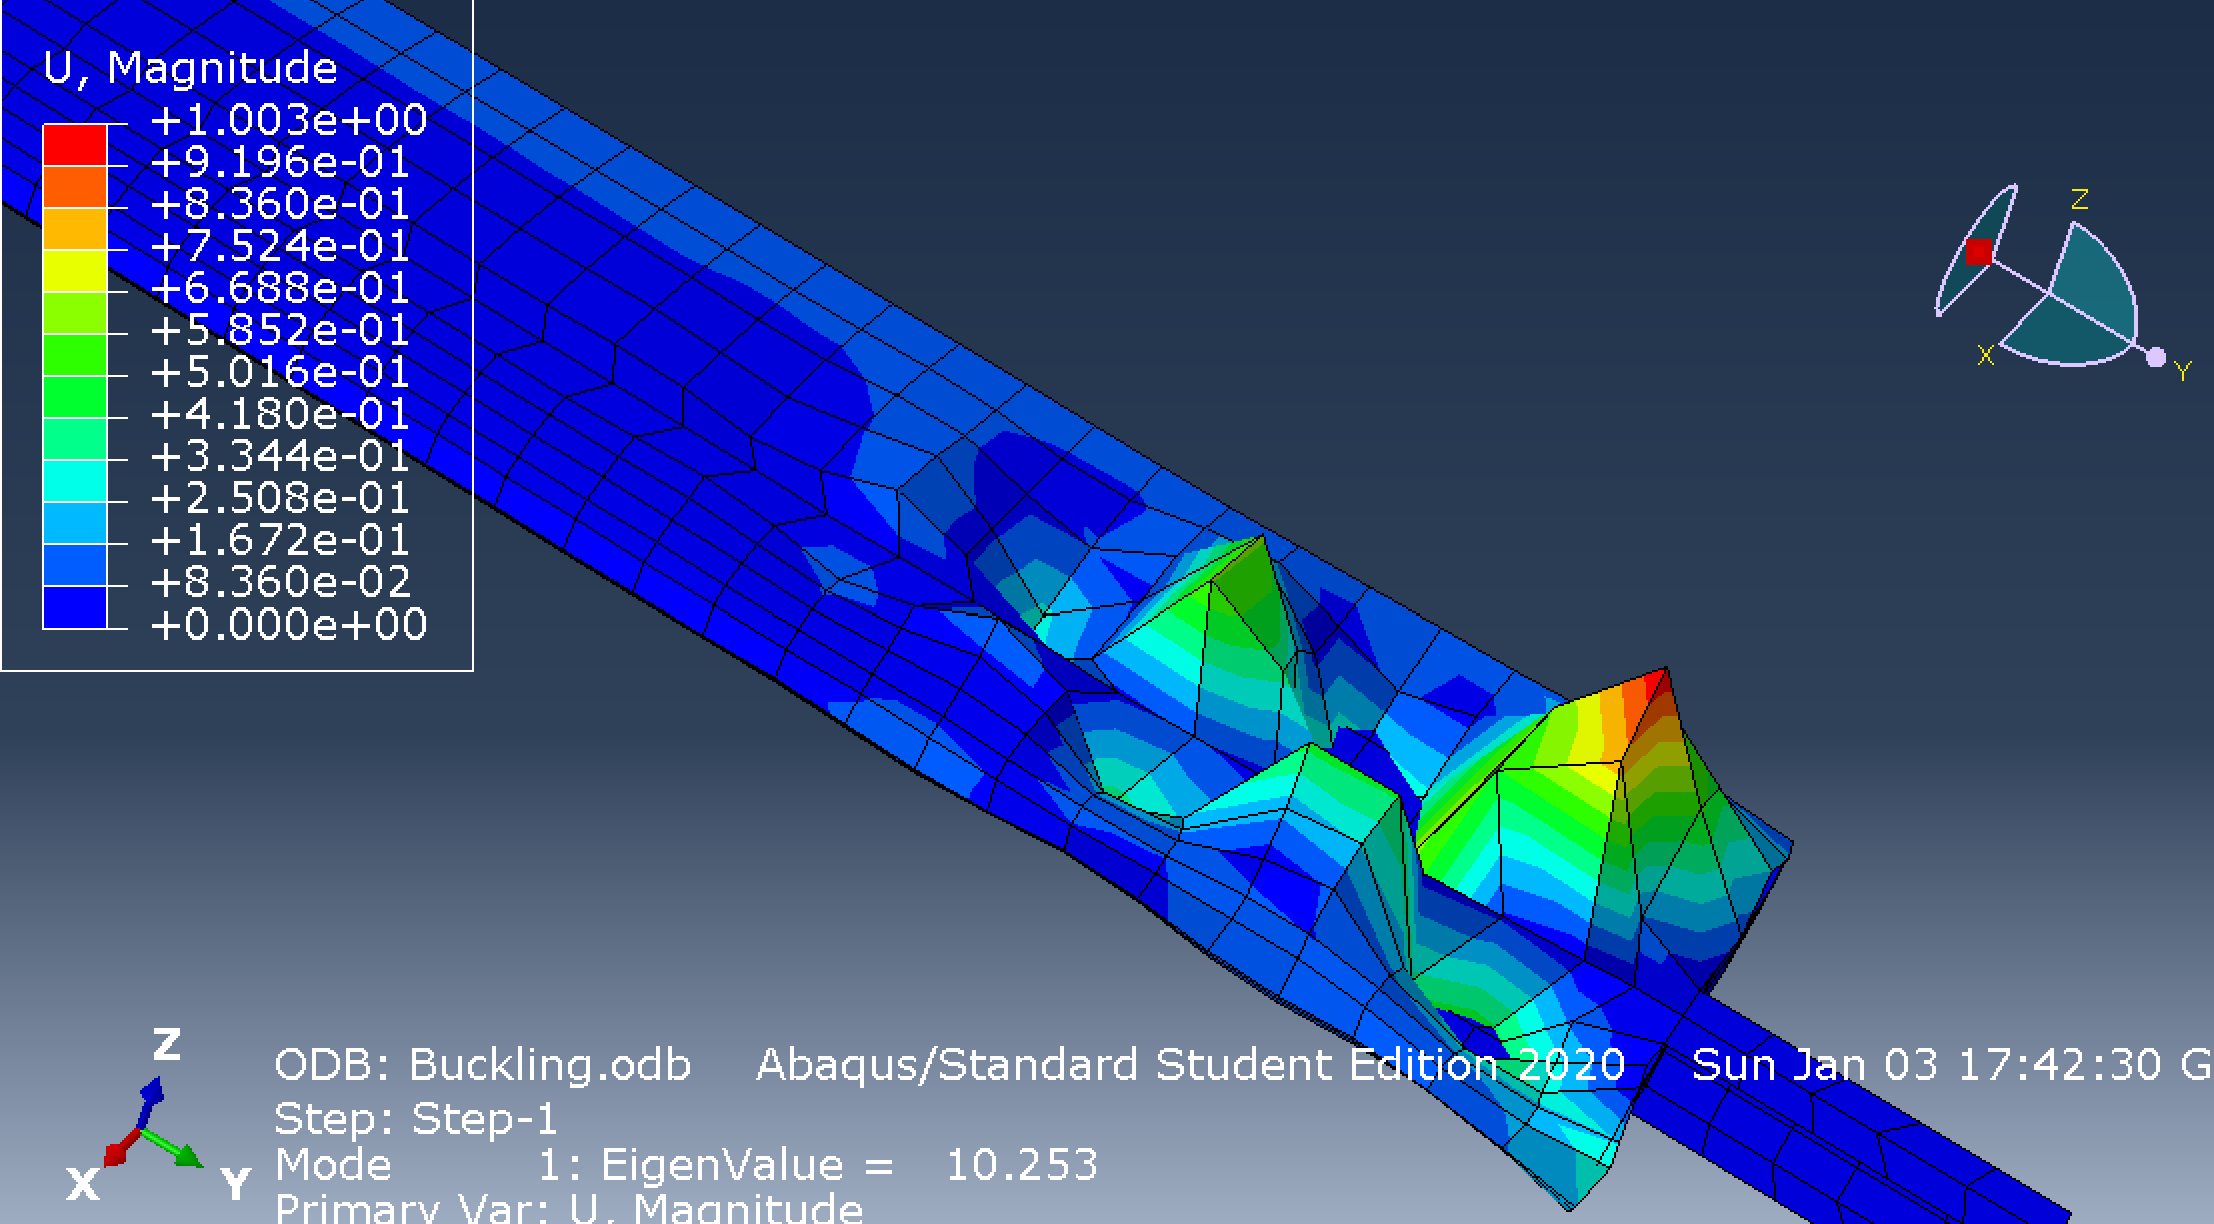
\includegraphics[scale=0.4]{Bilder/Beulen100N}
 \label{Beulform}
 \caption{Beispiel Beulform}
\end{figure}
\newpage

 

  
